\section{Evaluation}\label{s:eval}

We evaluate the following aspects of our design:
\begin{enumerate}
    \item To what extent can scheduling policies in \name improve performance?
    \item Is \name able to shift the bottleneck enough to enforce scheduling policies? We discuss this in \S\ref{s:robust}.
\end{enumerate}

\an{add backwards pointer to figure 1}

\radhika{Another way to structure the the rest of this section: /*}
\begin{itemize}
    \item Subsection: ``Understanding \name's performance benefits''. 
    \begin{itemize}
        \item (This will cover most of what you have under ``Flow Completion Time'')
        \item Experiment setup (what you currently have)
        \item Result: (Figure~\ref{fig:eval:best})
        \item Explaining why
        \begin{itemize}
            \item Effective bottleneck shifting: a graph that shows queuing delay at mahimahi without bundler, and graphs that show the queuing delay at mahimahi and inbox when using bundler. \an{(this is figure~\ref{fig:design:shift-bottleneck}, should we repeat it?)}
            \item Scheduling is necessary: comparison with FIFO -- what you have now
        \end{itemize}
        \item Comparison with ideal case: mahimahi link does sfq. Show we are not too bad (is it possible to get this result?). \an{will try, but it may not be possible to run sfq in mahimahi}
    \end{itemize}
    \item Subsection: ``Using \name to enforce different policies''.
    
    \begin{itemize}
        \item We use same set-up as before, but different scheduling and queue management polcies at the \name to meet different requirements. 
        \item Improved FCTs using FQ: Helps short flows achieve a smaller FCT by reducing the queuing delay that they see. Results already shown in previous subsection. 
        \item Smaller Queuing Delay using AQM: Helps keep queuing delay small. Present another FCT graph like Figure~\ref{fig:eval:best}, but with FQ-CoDel or PI. Also present a graph which shows the CDF of per-packet delays (if possible). Also, if possible (and if space), a comparison with properly configured and badly configured AQM scheme in the mahimahi link.
        \item Improved Rate Stability 
        \item Prioritizing interactive traffic
        \item anything else? 
    \end{itemize}
    \item Subsection: Robustness analysis
    \begin{itemize}
        \item We vary different aspects of the experiment setup detailed earlier to see how they impact our key results. We use SFQ as the scheduling policy in the bundler, but similar trends would hold for other policies (?). 
        \item Impact of congestion control (what you have now) [might also be fine if it goes in the previous subsection]
        \item Impact of offered load (what you have now)
        \item Impact of path characteristics
        \item Alternative design choices (TCP Proxy)
        \item Impact of cross traffic
        \begin{itemize}
            \item Cross traffic in it's own bundle
            \item Cross traffic not using bundle
        \end{itemize}
    \end{itemize}
\end{itemize}
\radhika{*/}


\subsection{Flow Completion Time}\label{s:eval:fct}
\radhika{another title for this section, or some preceding explanation on what each section is about}

\begin{figure}
    \centering
\begin{knitrout}
\definecolor{shadecolor}{rgb}{0.969, 0.969, 0.969}\color{fgcolor}
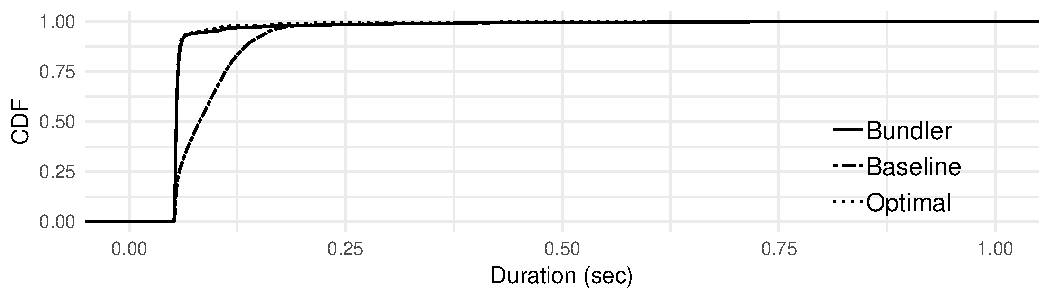
\includegraphics[width=\maxwidth]{figure/eval:best-1} 

\end{knitrout}
    \caption{\name achieves $33$\% lower median slowdown. Note the differing axis scales. For both \name and Optimal, performance benefits come from preventing short flows from queueing behind long ones. \an{Whiskers currently show 1.25 inter-quantile range, figure out how to show 99th \%ile? Also, can barely see Bundler and Optimal...}}
    \label{fig:eval:best}
\end{figure}


\paragrapha{Experiment Setup}
We evaluate our implementation of \name (discussed in \S\ref{s:impl}) using network emulation via mahimahi~\cite{mahimahi}.
\cut{\radhika{one-two lines explaining mahimahi? (can't expect reviewers to know about it / read the reference)} \an{should be fine to just say ``network emulator''?}}
There are three machines in our setup: one machine is a traffic generator, another is configured as a middlebox and runs an \inbox, and a third is the receiver. 
The out-box runs on the same machine as the receiver.
We run an empirical traffic generator, in which a many-threaded client on the receiver machine  generates requests from a given empirical request size CDF (described below) and sends them to one of $200$ server processes on the traffic generator.
 
Each server then responds to the client with the requested amount of data, and
we measure the flow completion time of each client request.
We use multiple server processes to emulate multiple machines behind the \name at the customer's edge that serve different client requests.
%
\cut{Note that it is important to use many server processes so that the effect of head-of-line blocking on the client requests is limited.
Indeed, all the CDFs presented in this section have a ``knee'' where the effects of head-of-line blocking become apparent.
}
\radhika{when the graphs are presented, explain the `knee' as an artifact of our expts caused due to some HoL blocking. Btw, are you sure that's why you have the knee?}

We first present results for a simplified scenario without any cross-traffic, i.e. all traffic traversing through the network is generated by the same customer and is, therefore, part of the same bundle. 
This scenario highlights the benefits of using \name when the congestion on the bottleneck link in the network is self-inflicted by a single customer. We later explore the effects of externally inflicted congestion, caused by other cross-traffic in \S\ref{s:robust}.

On a $96$Mbps link, we generate $84$Mbps of offered request load from a CDF with a heavy-tailed mix of short and long requests: 90\% of the requests are less than $5$KB, and 100\% of the requests are less than $1$MB.
In \S\ref{s:robust} we evaluate \name using a real-world request size CDF. 
Each CDF shown in this section is comprised of $100,000$ requests sampled from this distribution, across $10$ runs each with a different random seed.
In addition, there is a persistently backlogged connection inside the traffic aggregate that models a background large data transfer which would normally fill the bottleneck queue.

\paragrapha{Comparison with Optimal} 
Figure~\ref{fig:eval:best} presents the results with the above experiment setup.
We use a Copa~\cite{copa} congestion controller at the \inbox to manage the bottleneck queue, and the stochastic fair queueing~\cite{sfq} scheduling policy. 
We study the effects of different congestion control algorithms and different queuing policies in \S\ref{s:robust}.
With \name, the median 
slowdown\footnote{We define the ``slowdown'' of a request as its completion time divided by what its completion time would have been in an unloaded network. A slowdown of $1$ is optimal, and higher numbers represent worse performance.} 
decreases from $1.62$ using FIFO scheduling at the bottleneck link (we call this the baseline configuration as it represents the status quo) to $1.08$ with \name: 33\% lower.

Furthermore, \name's performance is near to the benefits that could be achieved by deploying scheduling on the bottleneck link (labelled ``Optimal''). 
We implement this scheme by modifying mahimahi (our patch comprises $171$ lines of C++) to add a packet-level fair-queueing scheduler to the bottleneck link.
Both \name and Optimal achieve an identical median slowdown of $1.08$.
The ``optimal'' configuration is more beneficial in the tail: the $99\%$ile slowdown is $4.46$ for ``optimal'' and $9.83$ for \name. Note that the baseline achieves a $99\%$ile slowdown of $10.77$.

Further, recall that this ``optimal'' configuration is not deployable in practice as we note in \S\ref{s:intro}: it forces \emph{all} customers, who may have diverging traffic characteristics, to use the same scheduling policy.

\vspace{10pt}
\noindent Where do these benefits come from? We devote the remainder of \S\ref{s:eval:fct} \radhika{this section} to exploring this question.

\paragrapha{Necessity of scheduling} It is important to note that \name by itself is not necessarily a means of achieving low end-to-end delays, as promised by recent efforts in congestion control~\cite{copa, nimbus}, despite its use of these modern congestion control algorithms. \an{forward pointer to fqcodel results}
To see why this is the case, recall that \name does not modify the end-hosts: they continue to run the default Cubic congestion controller, which will probe for bandwidth until it observes loss.
Indeed, the packets end-host Cubic sends beyond those the link can transmit must queue somewhere in the network or be lost. Without \name, they get queued up at the bottleneck link.
With \name, they instead queue at the \inbox.
However, the congestion controller at \inbox must also additionally maintain some standing queue at the bottleneck link to make decisions effectively.
Therefore, we expect the overall end-to-end-delays to increase slightly.
As a result, solely using a more sophisticated congestion control algorithm at the \name is unlikely to be the cause of significant reductions in the flow completion time.

\begin{figure}
    \centering
\begin{knitrout}
\definecolor{shadecolor}{rgb}{0.969, 0.969, 0.969}\color{fgcolor}
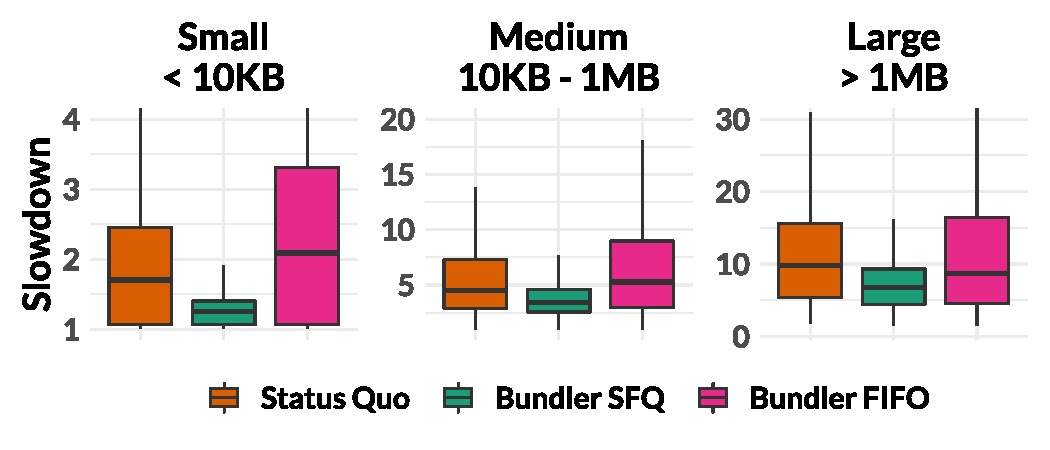
\includegraphics[width=\maxwidth]{figure/eval_fifo-1} 

\end{knitrout}
    \caption{With FIFO scheduling, the benefits of \name are lost: FCTs are 31\% worse in the median. Note the different y-axis scales for each group of request sizes.}
    \label{fig:eval:fifo}
\end{figure}
\newcommand{\overviewBenefitsFifoMedian}{2.13\xspace}
\newcommand{\overviewBenefitsFifoWorse}{31\%\xspace}


We can see this by measuring the relative performance of using FIFO scheduling at the \name instead of the SFQ scheduling in Figure~\ref{fig:eval:best}.
The results are in Figure~\ref{fig:eval:fifo}. 
Unsurprisingly, the FCTs with FIFO scheduling at \name are \emph{worse}: with a median FCT of $173$ms, it is $18$\% higher than the baseline. 

\radhika{need to further clean this.}

\radhika{seems like the rest of this section can go under robustness?}

\begin{figure}
    \centering
\begin{knitrout}
\definecolor{shadecolor}{rgb}{0.969, 0.969, 0.969}\color{fgcolor}
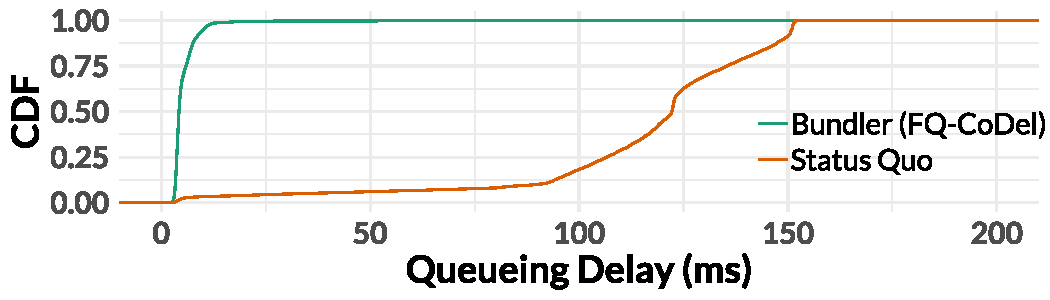
\includegraphics[width=\maxwidth]{figure/eval:lowdelays-1} 

\end{knitrout}
    \caption{We configure \name with the fq-codel scheduling policy to achieve low end-to-end queueing delays.}
    \label{fig:eval:lowdelays}
\end{figure}

\paragrapha{Achieving Low Delays}
\name can configure its scheduling policy to achieve low end-to-end-delays.
In Figure~\ref{fig:eval:lowdelays}, we show that when we configure the scheduling policy at \inbox, we can change the RTTs component connections obeserve.
Note that due to the effect discussed above, using FIFO scheduling results in higher delays than the baseline case.

\paragrapha{Impact of congestion control} How does our choice of congestion control impact our results? 
It is important to choose a congestion control algorithm carefully based on the known or inferred characteristics of the bottleneck link. 
In Figure~\ref{fig:eval:cc} we show three congestion control protocols: BBR~\cite{bbr}, Nimbus~\cite{nimbus}, and Copa~\cite{copa}.
In this scenario, it is important to control delays in the bottleneck queue, since it is FIFO scheduled and therefore queued packets from short requests must wait behind those from longer requests. Nimbus and BBR both maintain slightly higher queueing delays at the bottleneck link, and thus they achieve higher median FCTs \an{numbers}. 
Nimbus, which is slightly more aggressive than Copa, induces a higher queue build up at the bottleneck, and a smaller queue build up at the \name, when compared to Copa. It therefore results in a higher median FCT than Copa, though still providing significant benefits over the baseline. BBR, however is even more aggressive and cannot maintain sufficient queuing at the \name to provide enough benefits.

\radhika{Also, no way to further improve BBR?}

\an{try to understand bbr results}
\an{try running a cubic experiment}

\radhika{might be interesting to have another line that shows what happens when \name uses Cubic, and how it can break things.}
\an{I don't think we can run a meaningful cubic experiment since the implementation looks carefully at measurements (loss, out-of-order deliveries) that we don't precisely measure}

\begin{figure}
    \centering
\begin{knitrout}
\definecolor{shadecolor}{rgb}{0.969, 0.969, 0.969}\color{fgcolor}
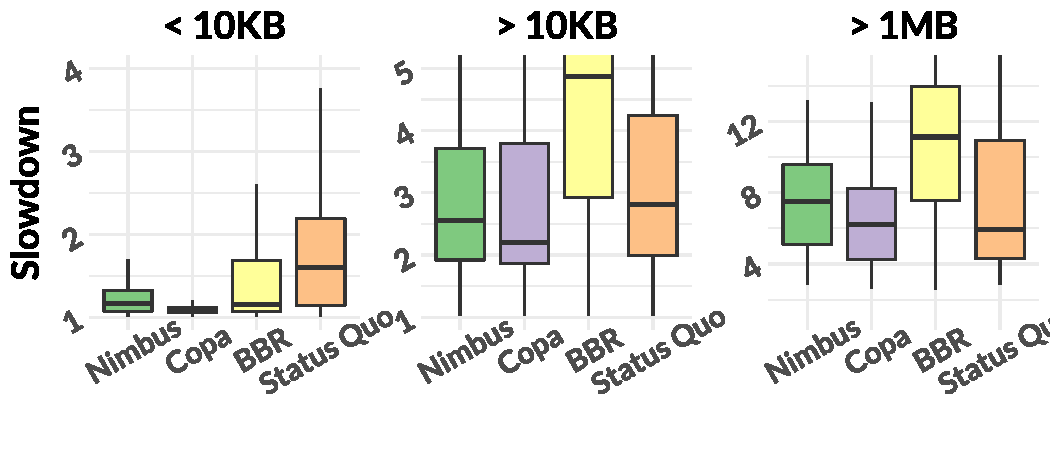
\includegraphics[width=\maxwidth]{figure/eval:cc-1} 

\end{knitrout}
    \caption{Choosing a congestion control algorithm at \name remains important, just as it is at the end-host. Note the different y-axis scales for each group of request sizes.}
    \label{fig:eval:cc}
\end{figure}
\newcommand{\ccCopaMedian}{}
\newcommand{\ccNimbusMedian}{}
\newcommand{\ccBBRMedian}{}
\newcommand{\ccBaselineMedian}{}


\paragrapha{Offered load} Naturally, if a link is less congested, scheduling the packets that traverse it will have less benefit. Accordingly, as we reduce the offered load in this experiment, we expect the gains from scheduling to diminish. The result is in Figure~\ref{fig:eval:offeredload}. We reduce the offered load by removing persistently backlogged connections from the workload and generating individual requests at 50\%, 75\% and 87.5\% of the bottleneck link bandwidth. 
At 87.5\% load, even without the load offered by a persistently backlogged connection, \name improves FCTs by \an{amount}. 
As the offered load decreases to 50\%, the benefit provided by \name decreases as well -- to \an{amount} at the 75th percentile.

\begin{figure*}[ht!]
    \centering
\begin{knitrout}
\definecolor{shadecolor}{rgb}{0.969, 0.969, 0.969}\color{fgcolor}
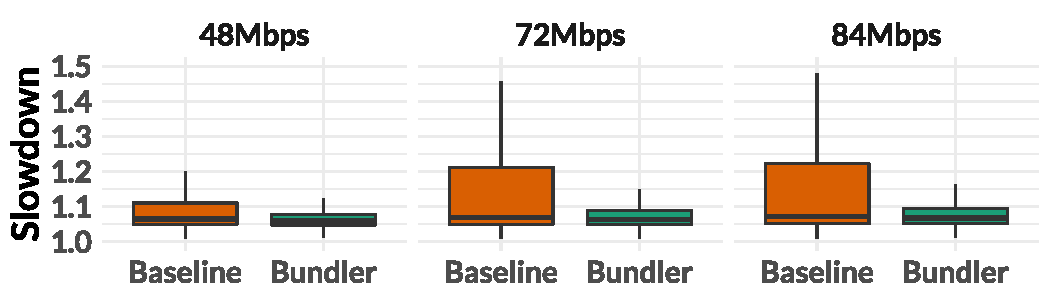
\includegraphics[width=\maxwidth]{figure/eval:offeredload-1} 

\end{knitrout}
    \caption{\name offers diminishing returns with lower amounts of offered load.}
    \label{fig:eval:offeredload}
\end{figure*}
%
%\newcommand{\highUtilTailImprove}{round(highUtilTailImprove, 0)\%\xspace}
%\newcommand{\medUtilTailImprove}{round(medUtilTailImprove, 0)\%\xspace}
%\newcommand{\lowUtilTailImprove}{round(lowUtilTailImprove, 0)\%\xspace}


\paragrapha{Terminating TCP Connections} An alternate implementation choice for a \name would use a TCP proxy to terminate connections at the \inbox. 
\radhika{I assume we mention this in an earlier section? else we need a line or two about why this experiment is interesting.}
We consider the best-case outcome of terminating TCP connections --- the effective RTT observed by the end-to-end congestion controller running at the servers would decrease (since the proxy would acknowledge its segments much faster than the original receiver would), and it would grow its window rapidly.
A proxy-based design would then apply scheduling policy to component traffic (recall that we use SFQ).
We emulate this best-case scenario by increasing the end-hosts' initial congestion window from the default $10$ to $1000$ segments.
Now, even the largest $1$MB ($\approx700$ packet) flows in this scenario can immediately transmit all their segments to the \inbox.
The result is in Figure~\ref{fig:eval:proxy}.

\begin{figure}
    \centering
\begin{knitrout}
\definecolor{shadecolor}{rgb}{0.969, 0.969, 0.969}\color{fgcolor}
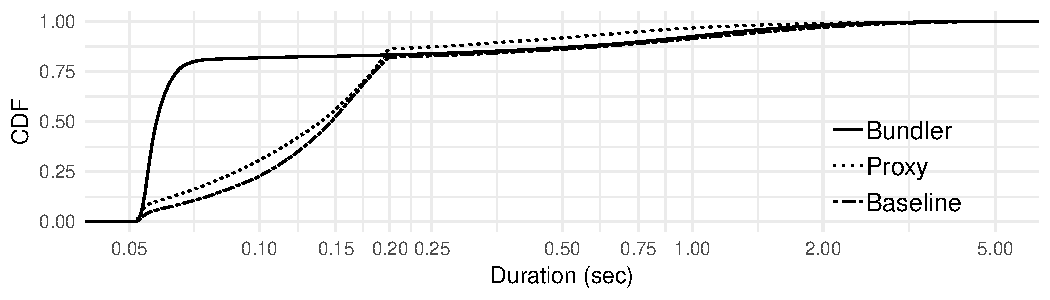
\includegraphics[width=\maxwidth]{figure/eval:proxy-1} 

\end{knitrout}
    \caption{Terminating TCP connections causes longer queues to build up at \inbox, and the resulting higher delays erase the gains of scheduling.}
    \label{fig:eval:proxy}
\end{figure}


Surprisingly, terminating TCP connections does not help the short flows (longer flows indeed see an improvement as expected). 
To see why, we refer back to Figure~\ref{fig:eval:fifo} --- absent scheduling, \name can cause performance degradation because it induces higher overall queueing delays.
In another instantiation of the same effect, rapid window growth from all active connections causes rapid queue growth at the \inbox. The resulting increased effect end-to-end delays and packet losses cancel out the gains of scheduling. \radhika{this might require a better explanation. let's discuss more in person.}

\subsection{Rate Stability}\label{s:eval:ratestable}

\begin{outline}
    \1 \name can improve the rate stability of component traffic
    \1 One such class of traffic is video streaming
\end{outline}
